\documentclass[a4paper, 12pt]{article}
\usepackage[utf8x]{inputenc}
\usepackage{cmap}
\usepackage[english, russian]{babel}
\usepackage{indentfirst}
\usepackage[left=20mm, top=20mm, right=20mm, bottom=20mm]{geometry}
\usepackage{tikz}
\usepackage{float}
\usepackage{amsmath, amsfonts, amssymb}
\usepackage{graphicx}
\usepackage{fancybox, fancyhdr}
\usepackage{hyperref}
\usepackage{listings}
\usepackage{caption}
\usepackage{subcaption}
\usepackage{xcolor}
\pagestyle{fancy}
\fancyhf{}
\fancyhead[L]{Домашнее задание №1}
\fancyhead[R]{Теоретическая вероятность}
\fancyfoot[C]{\thepage}
\graphicspath{{images/}}
\usetikzlibrary{patterns}
\definecolor{LightGray}{gray}{0.95}
\lstdefinestyle{pycode}{
    language=Python,
    basicstyle=\footnotesize\ttfamily,
    numbers=left,
    numberstyle=\tiny\color{gray},
    stepnumber=1,
    numbersep=5pt,
    backgroundcolor=\color{LightGray},
    showspaces=false,
    showstringspaces=false,
    showtabs=false,
    tabsize=4,
    captionpos=b,
    breaklines=true,
    breakatwhitespace=false,
    frame=none,
    rulecolor=\color{black},
    linewidth=\linewidth,
    keywordstyle=\color{red}\bfseries,
    commentstyle=\color{green!40!black},
    stringstyle=\color{blue},
    escapeinside={\%*}{*)},
    xleftmargin=0pt,
    framexleftmargin=0pt,
    framexrightmargin=0pt
}
\lstset{style=pycode}
\hypersetup{
    colorlinks=true,
    linkcolor=blue,
    filecolor=magenta,
    urlcolor=cyan,
    pdftitle={contents setup},
    pdfpagemode=FullScreen,
}
\setlength{\parskip}{1.5mm}
\setlength{\headheight}{15pt}
\setlength{\footskip}{15pt}
\allowdisplaybreaks
\DeclareMathOperator{\sinc}{sinc}
\newcommand{\frc}[2]{\raisebox{2pt}{$#1$}\big/\raisebox{-3pt}{$#2$}}

\begin{document}
    \begin{titlepage}

        \begin{center}
        
\includegraphics[width=0.3\textwidth]{itmo.png} % requires itmo.png in /images folder
        \vfill

        Федеральное государственное автономное образовательное учреждение высшего образования
        «Национальный Исследовательский Университет ИТМО»\\

        \vfill
        {\large\bf ДОМАШНЕЕ ЗАДАНИЕ №1}\\
        {\large\bf ПРЕДМЕТ «ТЕОРИЯ ВЕРОЯТНОСТЕЙ»}\\
        Вариант №1
        \vfill

        \begin{flushright}
            \begin{minipage}{.45\textwidth}
            {
                \hbox{Преподаватель:}
                \hbox{Шиманская Г. С.}
                \hbox{Студент:}
                \hbox{Румянцев А. А.}
                \hbox{}
                \hbox{Номер ИСУ:}
                \hbox{368731}
                \hbox{Поток:}
                \hbox{ТеорВер 1.2}
                \hbox{Факультет:}
                \hbox{СУиР}
                \hbox{Группа:}
                \hbox{R3241}
            }
            \end{minipage}
        \end{flushright}

        \vfill

        Санкт-Петербург\\
        2024
        \end{center}
    \end{titlepage}

    \tableofcontents

    \newpage
    \section{Задание 1.}
    \subsection{Условие.}
    Стержень сломан в двух случайно выбранных точках. Какова вероятность того, что из
    трех образованных отрезков можно сложить треугольник?


    \subsection{Решение.}
    Для решения задачи нам нужно знать, что треугольник существует только тогда,
    когда сумма его любых двух сторон больше третьей
    $$
    \exists\,\bigtriangleup \Leftrightarrow
    \begin{cases}
        a+b>c\\
        a+c>b\\
        b+c>a
    \end{cases}
    $$


    Пусть в нашем случае $l$ -- длина стержня, а $a,b \text{ и } c=l-a-b$ -- длины частей стержня после разлома.
    Очевидно, что $a,b,c>0$ и $b=l-a$ (второе следует из $a+b+c$, первое означает, что разлом точно был и мы получили
    части стержня). Следовательно, область возможных значений вероятности ограничена нулем и прямой $b$ и создает прямоугольник.
    \begin{figure}[H]
        \centering
        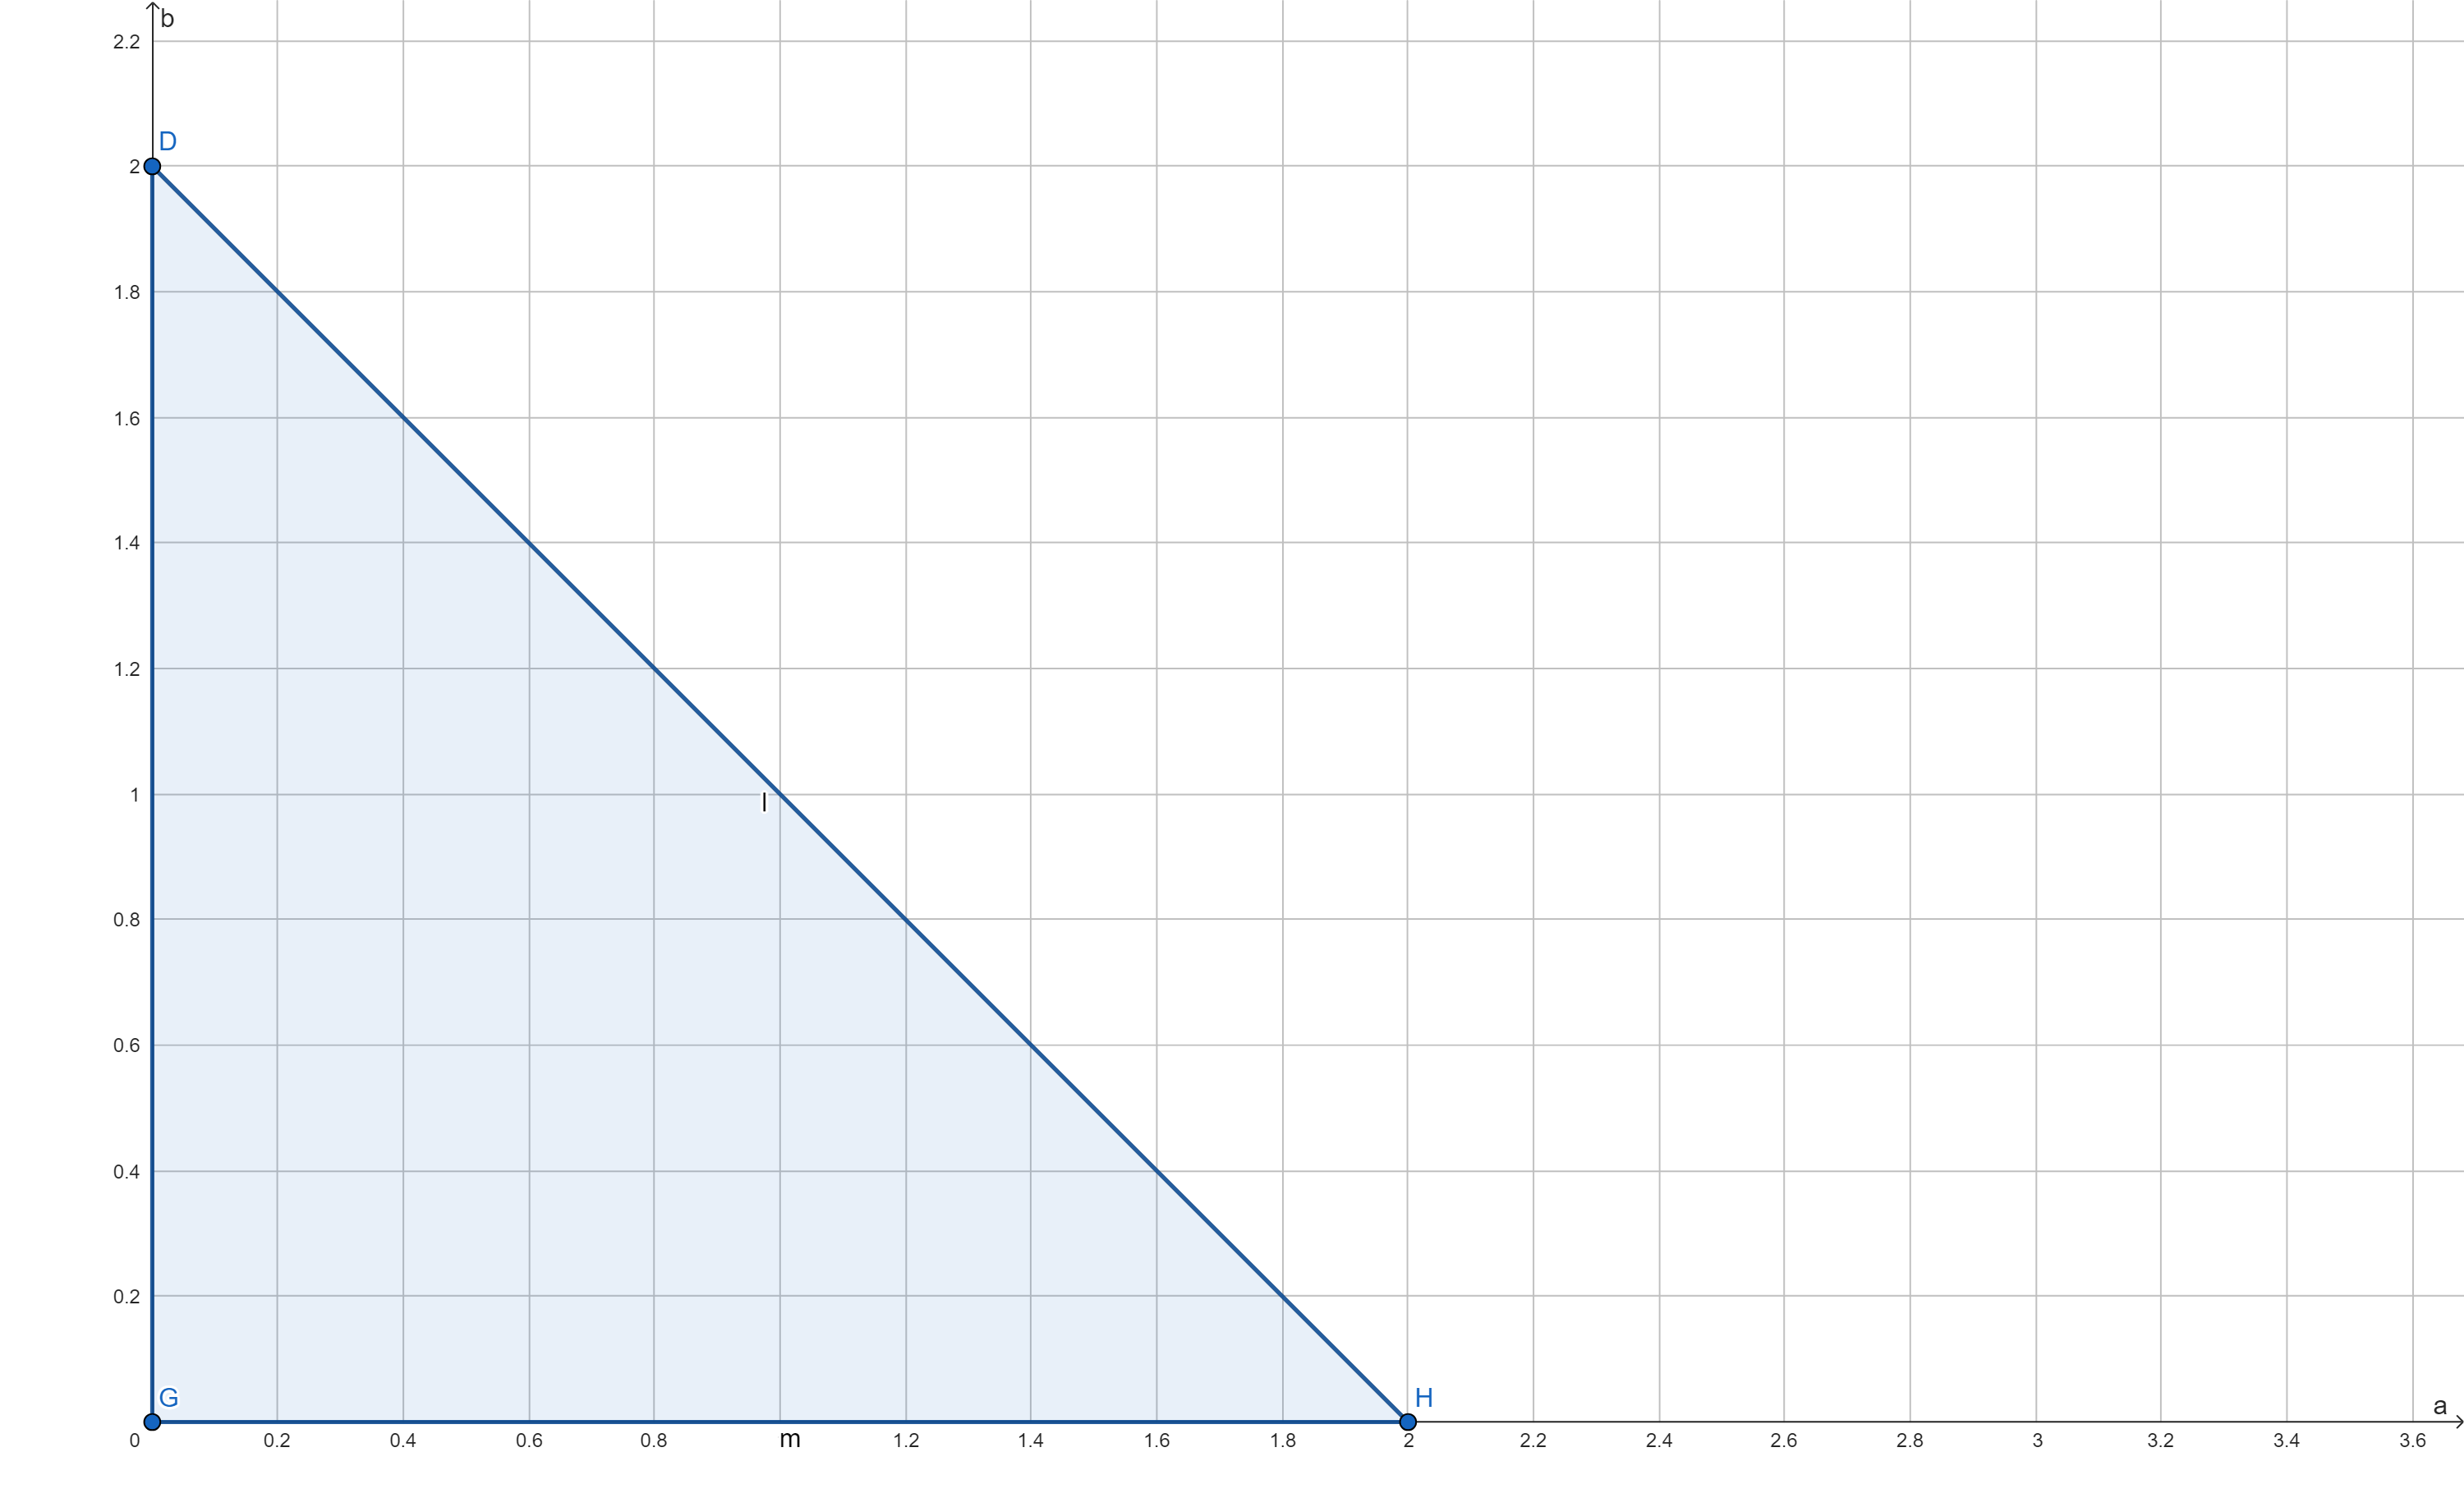
\includegraphics[scale=3]{show.png}
        \captionsetup{skip=0pt}
        \caption{Область возможных значений вероятности (для примера $l=2$).}
        \label{fig:show}
    \end{figure}


    Площадь области будет являться площадью прямоугольного треугольника (на рис. \ref{fig:show} видно, что при $l=2\Rightarrow a=b=2=l$):
    $$
    S=\dfrac{l^2}{2}
    $$


    Для того, чтобы составить из частей стержня треугольник, необходимо учесть два условия:
    $$
    \begin{cases}
        a,b<\frc{l}{2}\\
        a+b>\frc{l}{2}
    \end{cases}
    $$
    Область, которая удовлетворяет этому условию, лежит в треугольнике, который можно построить по прямым $a=\frc{l}{2},
    b={l}{2} \text{ и } a+b=\frc{l}{2}$.
    \begin{figure}[H]
        \centering
        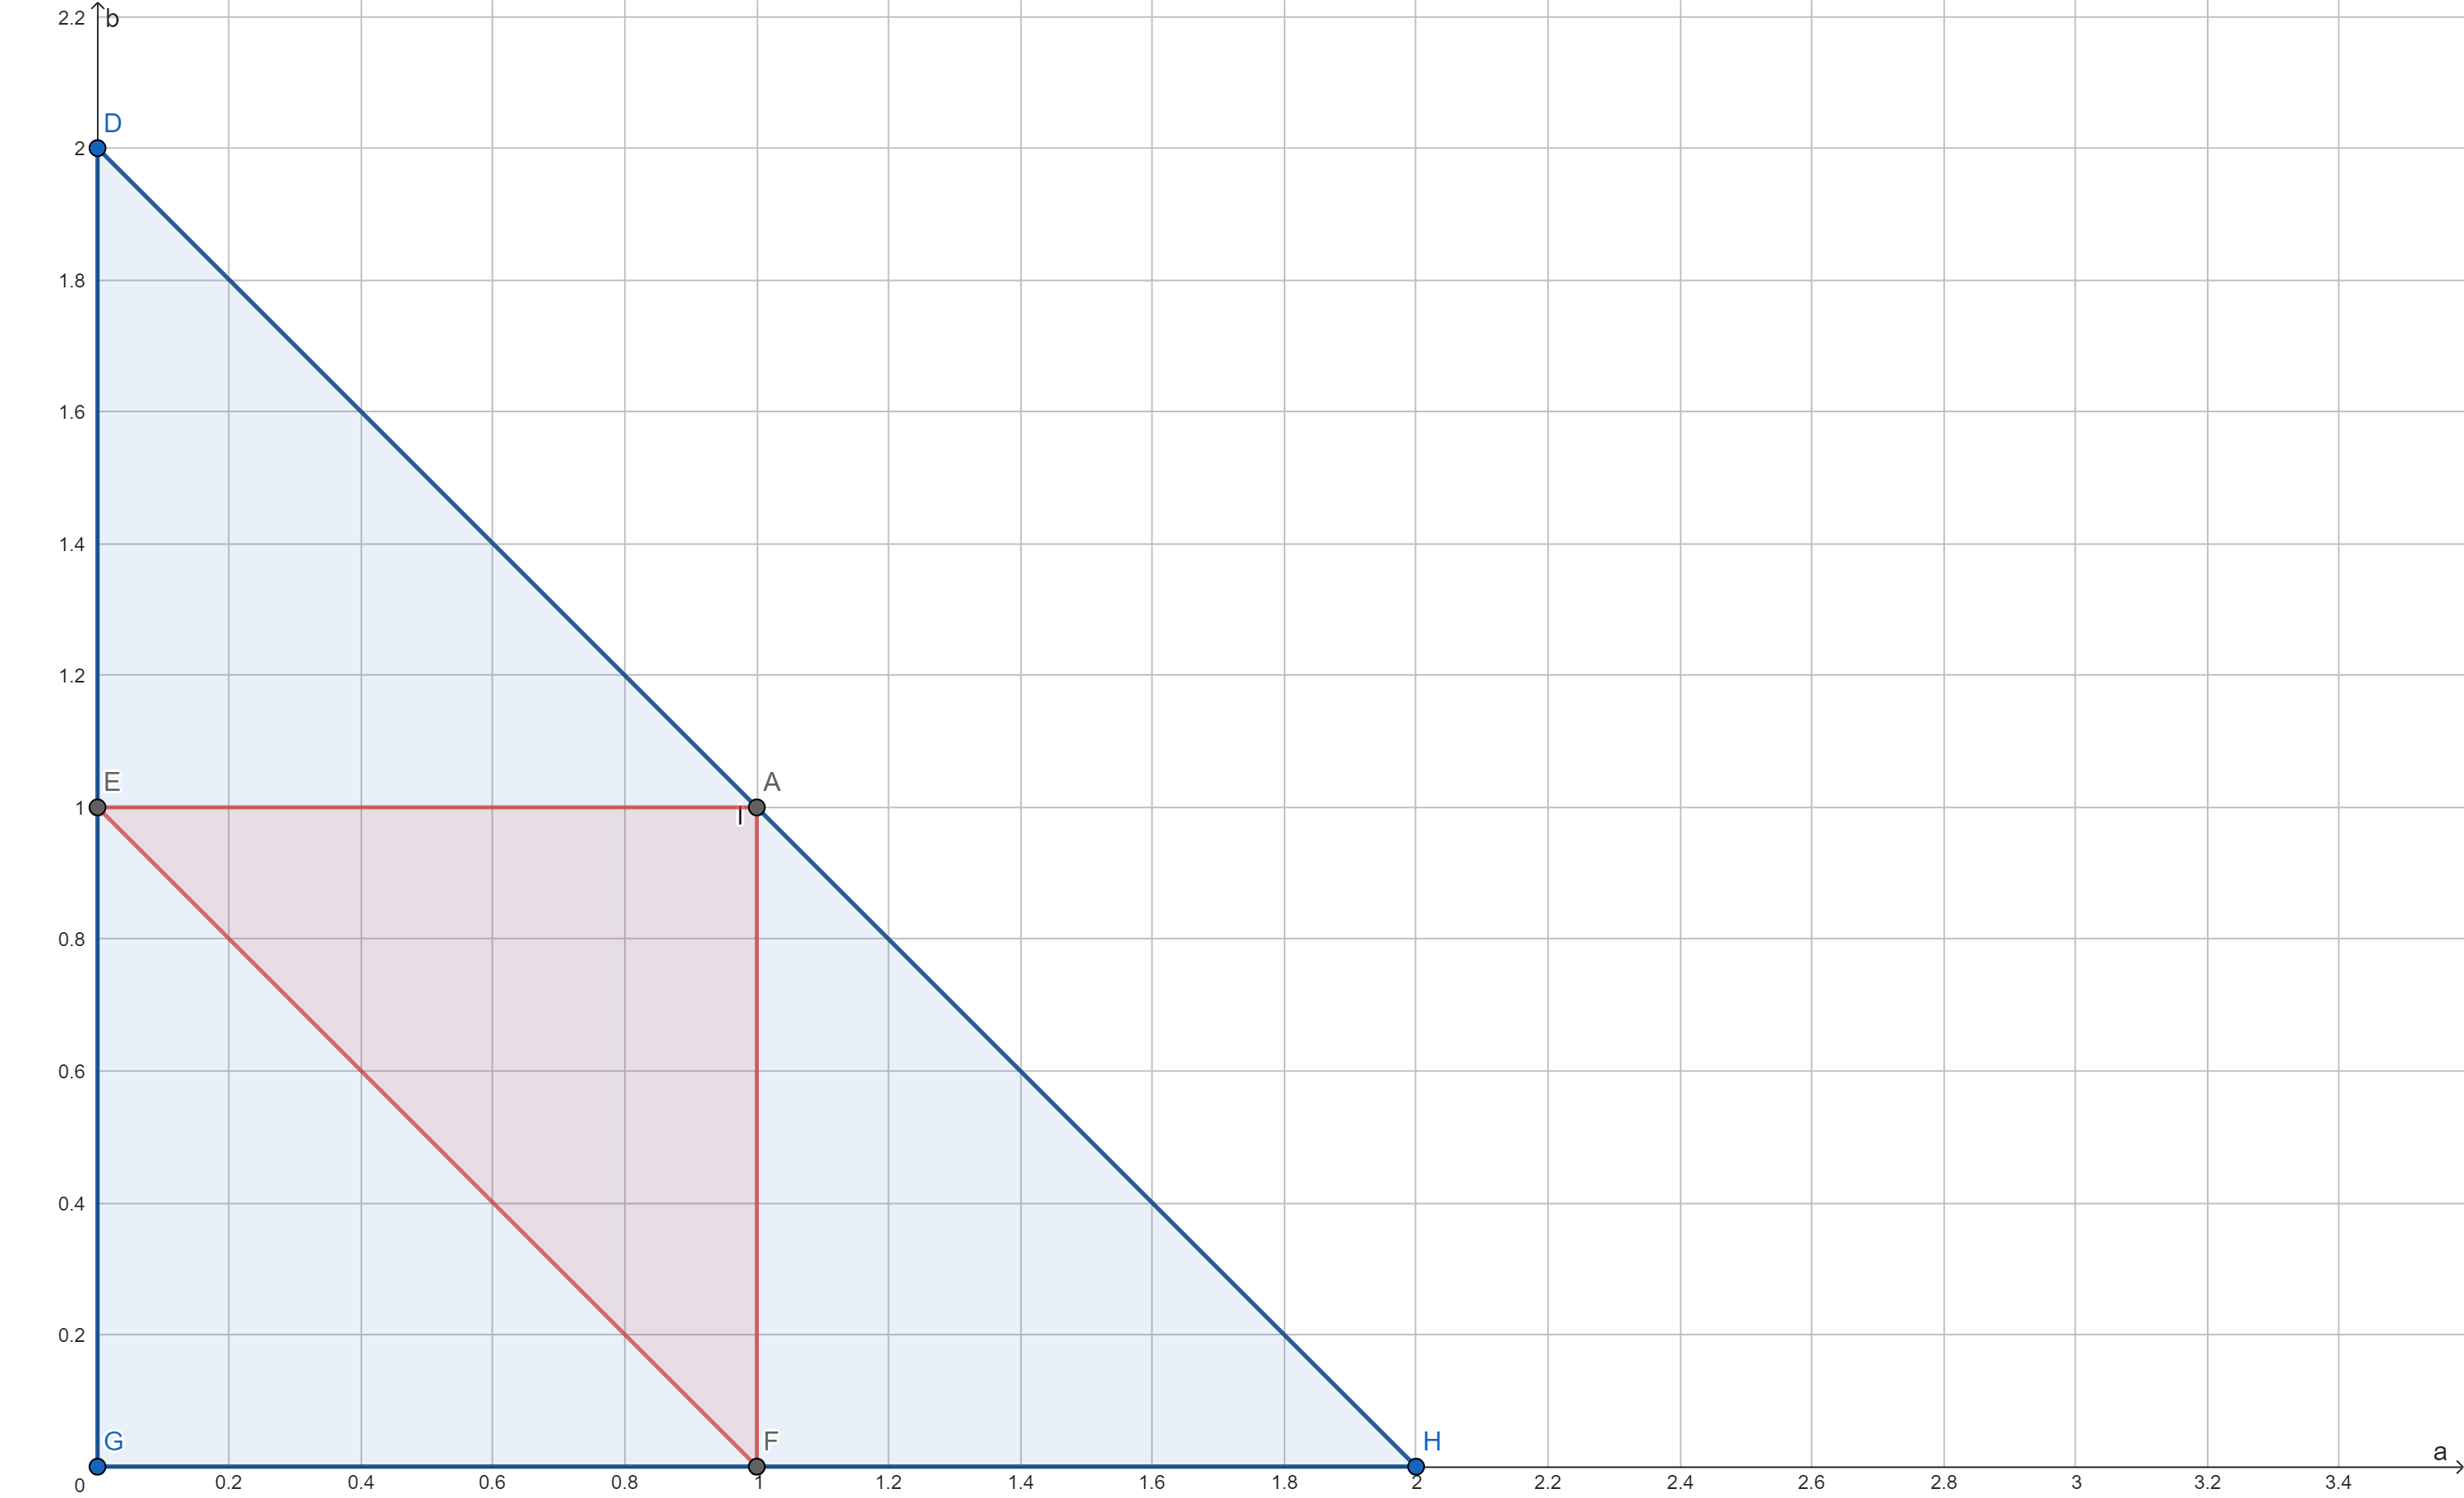
\includegraphics[scale=3]{show2.png}
        \captionsetup{skip=0pt}
        \caption{Область, удовлетворяющая условиям (для примера $l=2$).}
        \label{fig:show2}
    \end{figure}


    Площадь этого треугольника также будет определяться площадью прямоугольного треугольника, но уже со сторонами в 2 раза меньше $l$:
    $$
    S_{0}=\dfrac{\left(\frc{l}{2}\right)^2}{2}=\dfrac{l^2}{8}
    $$


    Таким образом, получим следующее соотношение, которое будет являться вероятностью интересующего нас события:
    $$
    P(S_0)=\dfrac{S_0}{S}=\dfrac{\frc{l^2}{8}}{\frc{l^2}{2}}=\dfrac{1}{4}
    $$

    
    \textbf{Ответ: $\mathbf{P(S_0)=0.25}$}


    \section{Задание 2.}
    \subsection{Условие.}
    В ящике имеются 10 монет по 20 коп., 5 монет по 15 коп. и 2 монеты по 10 коп. Наугад берутся
    шесть монет. Какова вероятность, что в сумме они составят не более одного рубля?


    \subsection{Решение.}
    Для выполнения этого задания нам понадобится формула сочетаний $$C_{n}^{k}=\dfrac{n!}{(n-k)!\,k!},$$
    где сочетание из $n$ по $k$ является неупорядоченным набором из $k$ различных элементов, взятых из некоторого множества
    с мощностью $n$, где $k\leq n$.


    Пойдем от обратного. Найдем все возможные случаи, когда сумма выбранных монет превышает 1 рубль:
    $$
    6\cdot20;\ 5\cdot 20 + 1\cdot 15;\ 5\cdot20 + 1\cdot 10;\ 4\cdot 20 + 2\cdot 15;\ 3\cdot 20 + 15\cdot 3;\ 4\cdot20 + 1\cdot 15 + 1\cdot 10 \geq 1
    $$
    Теперь распишем каждый случай сочетаниями. Сумма монет будет равносильна умножению соответствующих сочетаний. Всего берем $6$ монет из 17:
    $$
    \dfrac{C_{10}^{6}}{C_{17}^{6}};\ \dfrac{C_{10}^{5}\cdot C_{5}^{1}}{C_{17}^{6}};\ \dfrac{C_{10}^{5}\cdot C_{2}^{1}}{C_{17}^{6}};\ \dfrac{C_{10}^{4}\cdot C_{5}^{2}}{C_{17}^{6}};
    \ \dfrac{C_{10}^{3}\cdot C_{5}^{3}}{C_{17}^{6}};\ \dfrac{C_{10}^{4}\cdot C_{5}^{1}\cdot C_{2}^{1}}{C_{17}^{6}}
    $$
    Объясню смысл на примере $(C_{10}^{4}\,C_{5}^{1}\,C_{2}^{1})\div C_{17}^{6}$ -- берем в любом порядке 4 монеты по 20 копеек из 10 существущих,
    1 монету из 5 по 15 копеек и 1 монету из 2 по 10 копеек. Делим на то, сколько монет берем из скольки -- 6 монет из 17. Порядок не имеет значения, например, мы
    можем сначала взять 2 монеты по 20, потом 1 по 10, потом две по 20, потом 1 по 15.


    Так как мы идем от обратного, то нужно из единицы вычесть сумму всех сочетаний, описанных ранее, тогда имеем:
    $$
    1-\dfrac{1}{C_{17}^{6}}\left(C_{10}^{6}+C_{10}^{5}\,C_{5}^{1}+C_{10}^{5}\,C_{2}^{1}+C_{10}^{4}\,C_{5}^{2}+C_{10}^{3}\,C_{5}^{3}+C_{10}^{4}\,C_{5}^{1}\,C_{2}^{1}\right)
    $$
    Каждое сочетание считается по формуле, приведенной ранее, поэтому распишем только одно сочетание как пример расчета:
    $$
    C_{10}^{4}\,C_{5}^{1}\,C_{2}^{1}=\dfrac{10!}{6!\,4!}\cdot\dfrac{5!}{4!}\cdot 2!=2100
    $$
    Наконец получим
    $$
    1-\dfrac{1}{12376}\left(210+1260+504+2100+1200+2100\right)=1-\dfrac{7374}{12376}=\dfrac{2501}{6188}\approx 0.4
    $$


    \textbf{Ответ: $\mathbf{P(A)\approx 0.4}$}

    
    \section{Задание 3.}
    \subsection{Условие.}
    Доказать, что
    \begin{align*}
    & P\left(\prod_{k=1}^{n}A_k\right)=\sum\limits_{k=1}^{n}P\left(A_k\right)-\sum\limits_{k=1}^{n-1}\sum\limits_{j=k+1}^{n}
    P\left(A_k+A_j\right)+\\ &+\sum\limits_{k=1}^{n-2}\sum\limits_{j=k+1}^{n-1}\sum\limits_{i=j+1}^{n}P\left(A_k+A_j+A_i\right)
    -\hdots\\ & \hdots +\left(-1\right)^{n-1}P\left(\sum\limits_{k=1}^n A_k\right)
    \end{align*}


    \subsection{Решение.}
    Докажем от обратного. Сначала проверим, выполняется ли выражение для наименьшего значения перменной:
    $$
    P(A_1)=P(A_1)
    $$
    Очевидно, что выполняется. Теперь предположим, что выражение верно для $n=m$:
    \begin{align*}
        & P\left(\prod_{k=1}^{m}A_k\right)=\sum\limits_{k=1}^{m}P\left(A_k\right)-\sum\limits_{k=1}^{m-1}\sum\limits_{j=k+1}^{m}
        P\left(A_k+A_j\right)+\\ &+\sum\limits_{k=1}^{m-2}\sum\limits_{j=k+1}^{m-1}\sum\limits_{i=j+1}^{m}P\left(A_k+A_j+A_i\right)
        -\hdots\\ & \hdots +\left(-1\right)^{m-1}P\left(\sum\limits_{k=1}^m A_k\right)
    \end{align*}


    Докажем равенство выражений для $n=m+1$. Для этого рассмотрим $P\left(\prod_{k=1}^{m+1}A_k\right)$.
    Воспользуемся определением условной вероятности и запишем формулу следующим образом:
    $$
    P\left(\prod_{k=1}^{m+1}A_k\right)=P\left(A_{m+1}\cap \prod_{k=1}^{m}A_k\right)
    $$
    Далее применим формулу включений-исключений для двух событий:
    $$
    P\left(A_{m+1}\cap \prod_{k=1}^{m}A_k\right)=P(A_{m+1})+P\left(\prod_{k=1}^{m}A_k\right)-P\left(A_{m+1}+\prod_{k=1}^{m}A_k\right)
    $$
    Известно, что $P\left(A_{m+1}+\prod_{k=1}^{m}A_{k}\right)$ является объединением событий, аналогичным их умножению:
    \begin{align*}
    &P\left(A_{m+1}\cap \prod_{k=1}^{m}A_k\right)=\sum\limits_{k=1}^{m}P(A_{m+1}+A_{k})-\sum\limits_{k=1}^{m-1}\sum\limits_{j=k+1}^{m}P(A_{m+1}+A_{k}+A_{j})
    +\hdots\\ &\hdots +(-1)^{m-1}P\left(\sum\limits_{k=1}^{m}A_{m+1}+A_{k}\right)
    \end{align*}
    Осталось подставить это обратно в наше выражение:
    \begin{align*}
        & P\left(\prod_{k=1}^{m+1}A_k\right)=P(A_{m+1})+P\left(\prod_{k=1}^{m}A_{k}\right)-\left[\sum\limits_{k=1}^{m}P(A_{m+1}+A_{k})+\right.\\
        & \left.-\sum\limits_{k=1}^{m-1}\sum\limits_{j=k+1}^{m}P(A_{m+1}+A_{k}+A_{j})+\hdots+(-1)^{m-1}P\left(\sum\limits_{k=1}^{m}A_{m+1}+A_{k}\right)\right]
    \end{align*}
    После преобразований мы получим формулу включений-исключений для $n=m+1$, что завершает наше доказательство от обратного.

    
    \textbf{Что и требовалось доказать}


    \section{Задание 4.}
    \subsection{Условие.}
    Третья часть одной из трех партий деталей является второсортной, остальные детали первого сорта. Деталь, взятая из одной партии,
    оказалась первосортной. Определить вероятность того, что деталь была взята из партии, имеющей второсортные детали. Найти ту же
    вероятность при условии, что взятая из той же партии вторая деталь оказалась первосортной, если первая деталь после проверки 
    возвращена в партию.


    \subsection{Решение.}
    Для решения этого задания нам понадобится формула Байеса, которая имеет вид
    $$P\left(B_i | A\right)=\dfrac{P\left(A | B_i\right)P\left(B_i\right)}{\sum\limits_{j=1}^{N}P\left(A|B_{j}\right)P\left(B_j\right)}$$ и является
    соотношением различных предполагаемых вероятностей различных событий, которое дает вероятность, что какое-то
    событие $A$ является результатом $X$ ряда независимых друг от друга событий $B_1,B_2\hdots B_n$, который,
    возможно, привел к $A$. Обозначения следующие: $P\left(A\right)$ -- вер. события $A$, $P\left(A|B\right)$ -- вер. события $A$ при
    наступлении события $B$, $P\left(B|A\right)$ -- вер. наступления события $B$ при истинности события $A$, $P\left(B\right)$ --
    вероятность наступления события $B$.


    Составим событие и гипотезы:
    \begin{enumerate}
        \item $A$ -- выбранная деталь первого сорта
        \item $H_1$ -- деталь из первой партии
        \item $H_2$ -- деталь из второй партии
        \item $H_3$ -- деталь из третьей партии
    \end{enumerate}


    Представим, что именно первая партия содержит детали второго сорта. Тогда вероятность вытащить деталь первого сорта из
    партии, содержащей второй сторт вычисляется по формуле $$P\left(A|H_1\right)=\dfrac{2}{3},$$ так как только треть деталей
    является вторым сортом. Определим вероятность вытащить первый сорт из второй и третьей партий:
    $$
    P\left(A|H_2\right)=P\left(A|H_3\right)=1
    $$
    По условию другие партии не содержат детали второго сорта, поэтому вероятности равны единице. Теперь найдем вероятность
    выбрать партию именно с деталями второго сорта:
    $$
    P(H_1)=P(H_2)=P(H_3)=\dfrac{1}{3}
    $$
    Очевидно, что вероятности равны, так как мы выбираем лишь одну партию из трех один раз. Эта вероятность не зависит от предположения,
    в какой именно партии содержатся детали второго сорта, так как по сути они могут содержаться в любой из них, мы лишь условились, что
    они именно в первой, мы создали гипотезу.


    Найдем полную вероятность события $A$ для всех гипотез:
    $$
    P(A)=P(A|H_1)P(H_1)+P(A|H_2)P(H_2)+P(A|H_3)P(H_3)=\dfrac{1}{3}\left(\dfrac{2}{3}+1+1\right)=\dfrac{8}{9}
    $$
    Осталось найти искомую вероятность по формуле Байеса:
    $$
    P(H_1|A)=\dfrac{P(A|H_1)P(H_1)}{P(A)}=\dfrac{\frc{2}{3}\cdot\frc{1}{3}}{\frc{8}{9}}=\dfrac{1}{4}
    $$


    Перейдем ко второму пункту. У нас остались те же гипотезы, но теперь условие такое -- мы берем из первой партии (мы ее взяли за
    партию с второсортными деталями) одну первосортную деталь, возвращаем, а потом берем оттуда же еще одну деталь первого сорта.
    Так как количество деталей не изменилось, наши вероятности выбрать детали изменятся следующим образом:
    $$
    P(A^2|H_1)=\dfrac{2}{3}\cdot\dfrac{2}{3}=\dfrac{4}{9},\ P(A^2|H_2)=P(A^2|H_3)=1^2=1.
    $$
    А формула полной вероятности будет иметь вид:
    $$
    P(A)=P(A^2|H_1)P(H_1)+P(A^2|H_2)P(H_2)+P(A^2|H_3)P(H_3)=\dfrac{1}{3}\left(\dfrac{4}{9}+1+1\right)=\dfrac{22}{27}
    $$
    Тогда формула Байеса примет следующий вид:
    $$
    P(H_1|A^2)=\dfrac{P(A^2|H_1)P(H_1)}{P(A^2)}=\dfrac{\frc{4}{9}\cdot\frc{1}{3}}{\frc{22}{27}}=\dfrac{2}{11}\approx 0.18
    $$


    \textbf{Ответ: $\mathbf{P(H_1|A)=0.25,\ P(H_1|A^2)\approx0.18}$}

    
    \section{Задание 5.}
    \subsection{Условие.}
    Найти наивероятнейшие числа отрицательных и положительных ошибок и соответствующую вероятность при четырех измерениях, если
    при каждом измерении вероятность получения положительной ошибки равна $\frc{2}{3}$, а отрицательной -- $\frc{1}{3}$


    \subsection{Решение.}
    Распределение по схеме Бернулли позволяет установить, какое число появлений события A наиболее вероятно. Формула для
    наиболее вероятного числа успехов $k$ (появлений события) имеет вид $$np-q\leq k \leq np+p,\ q=1-p,$$ причем вследствие
    выполнения равенства $$np-q=np+p-1$$ границы отличаются на $1$, поэтому $k\in \mathbb{Z}$.


    Рассмотрим случай с положительными ошибками. Мы знаем, что $n=4$. Пусть $p=\frc{2}{3}$, тогда $q=\frc{1}{3}$. Формула примет вид
    $$4\cdot\dfrac{2}{3}-\dfrac{1}{3}\leq k_{+}\leq 4\cdot \dfrac{2}{3}+\dfrac{2}{3}\Rightarrow \dfrac{7}{3}\leq k_{+} \leq \dfrac{10}{3}.$$
    Так как рациональные числа намм не подходят, берем $k_{+}=\frc{9}{3}=3$. Теперь можем найти соответствующую вероятность $P\left(K=k\right)$:
    $$
    P\left(K=k\right)=C_{n}^{k}\,p^{k}\,q^{n-k}\Rightarrow P\left(K=3\right)=C_{4}^{3}\,p^{3}\,q^{4-3}=\dfrac{4!}{3!}\cdot\left(\dfrac{2}{3}\right)^{3}\cdot\dfrac{1}{3}=\dfrac{32}{81}
    $$


    Аналогичные действия для случая с отрицательными ошибками, однако теперь зададим $p=\frc{1}{3},\,q=\frc{2}{3}$:
    $$
    4\cdot\dfrac{1}{3}-\dfrac{2}{3}\leq k_{-}\leq 4\cdot\dfrac{1}{3}+\dfrac{1}{3}\Rightarrow\dfrac{2}{3}\leq k_{-} \leq \dfrac{5}{3}\Rightarrow k_{-}=1
    $$
    $$
    P\left(K=1\right)=C_{4}^{1}\,p^{1}\,q^{4-1}=\dfrac{4!}{3!}\cdot\dfrac{1}{3}\cdot\left(\dfrac{2}{3}\right)^3=\dfrac{32}{81}
    $$
    Как видим, вероятности совпали $(P(K=3)=P(K=1))$, значит все верно.


    \textbf{Ответ: $\mathbf{k_{+}=3,\ k_{-}=1,\ P=\dfrac{32}{81}}$}
\end{document}